\section{Methodology}
\label{sec:vibvoice_method}
In this section, we first develop EarSense, an open-source wearable platform that has a similar setup to current commercial HMWs for data collection in Section. \ref{sec:vibvoice_EarSense}. Then, we exploit the bone-conducted vibrations and the audio signals recorded by EarSense under various settings in Section. \ref{sec:vibvoice_measurement}. Finally, we overview the design of our proposed system in Section. \ref{sec:vibvoice_overview}, introduce Bone Conduction Function and multi-modal network in Section. \ref{sec:vibvoice_bcf} and Section. \ref{sec:vibvoice_network}, respectively.


\subsection{EarSense: An Open Source Data Collection Platform for HMWs}
\label{sec:vibvoice_EarSense}

Most commercial HMWs do not provide APIs to collect raw acceleration data. Recently, Apple provided APIs \citep{CMHeadph3:online} to collect motion data from AirPods earphones at $100\,\text{Hz}$, which is too low for speech recording and doesn't fully utilize commercial IMU.
Hence, it is desirable to develop a new sensing platform that can: a) collect the acceleration and acoustic data synchronously at a sample rate to recover speech information; b) have direct contact with the user's head like HMWs; c) have compatibility to test with existing commercial devices.
\begin{figure}
  \begin{subfigure}{.64\columnwidth}
    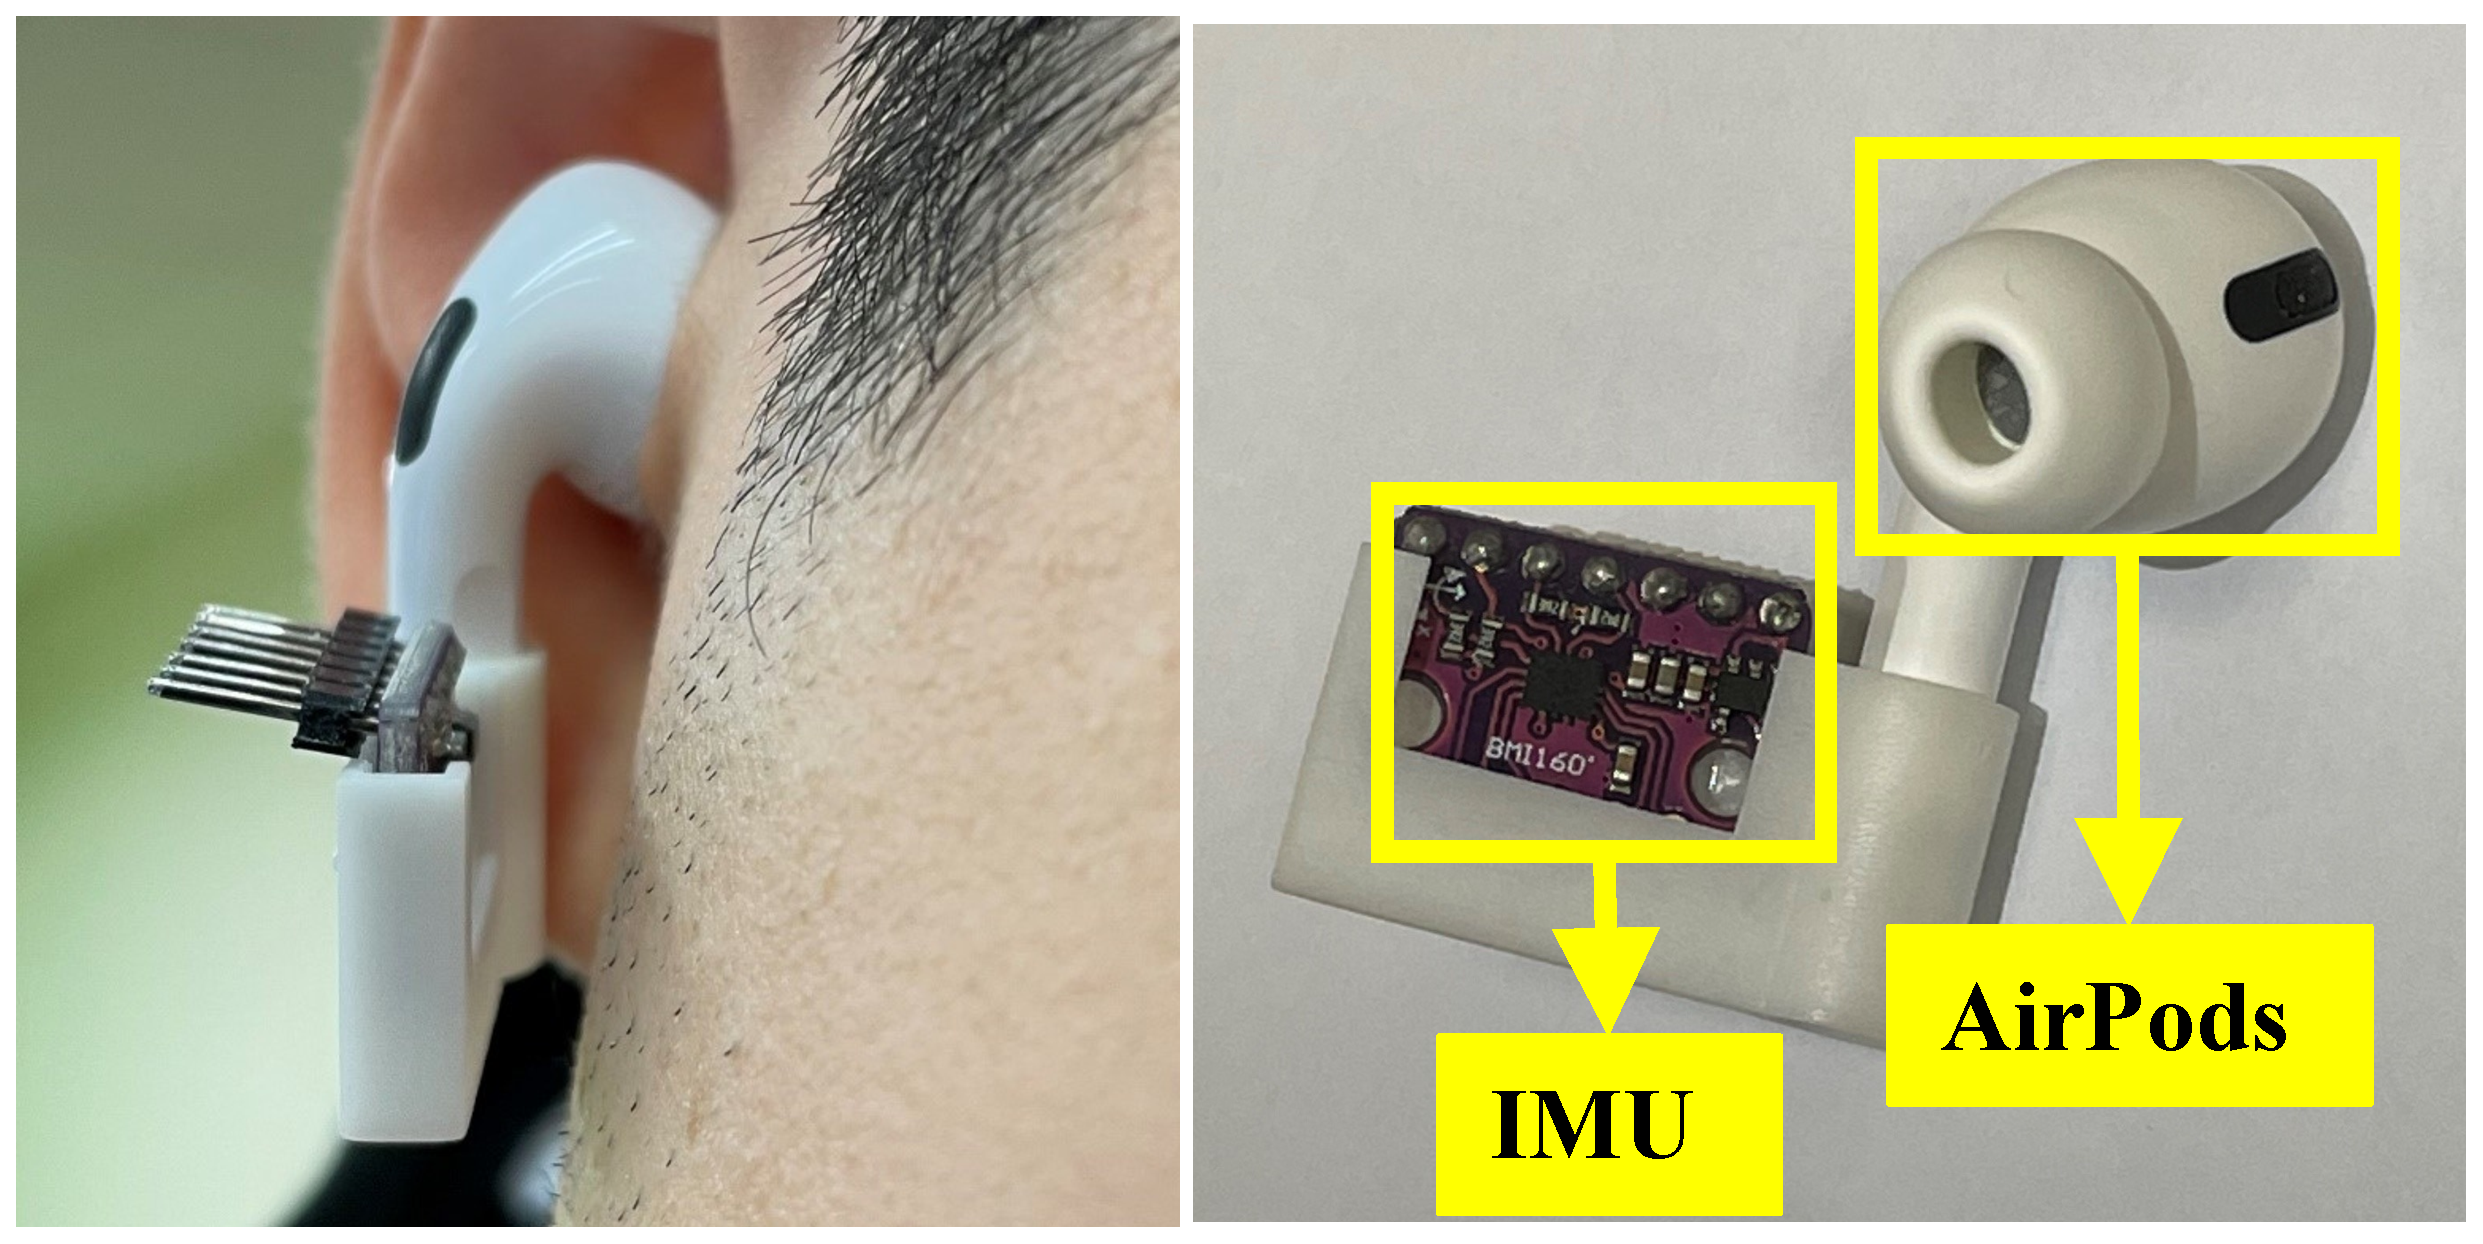
\includegraphics[width=\textwidth]{chapters/vibvoice/figure/earsense.eps}
    \caption{\emph{EarSense} with an Airpods Pro.}
    \label{fig:vibvoice_earsense-head}
  \end{subfigure}
  \begin{subfigure}{0.35\columnwidth}
    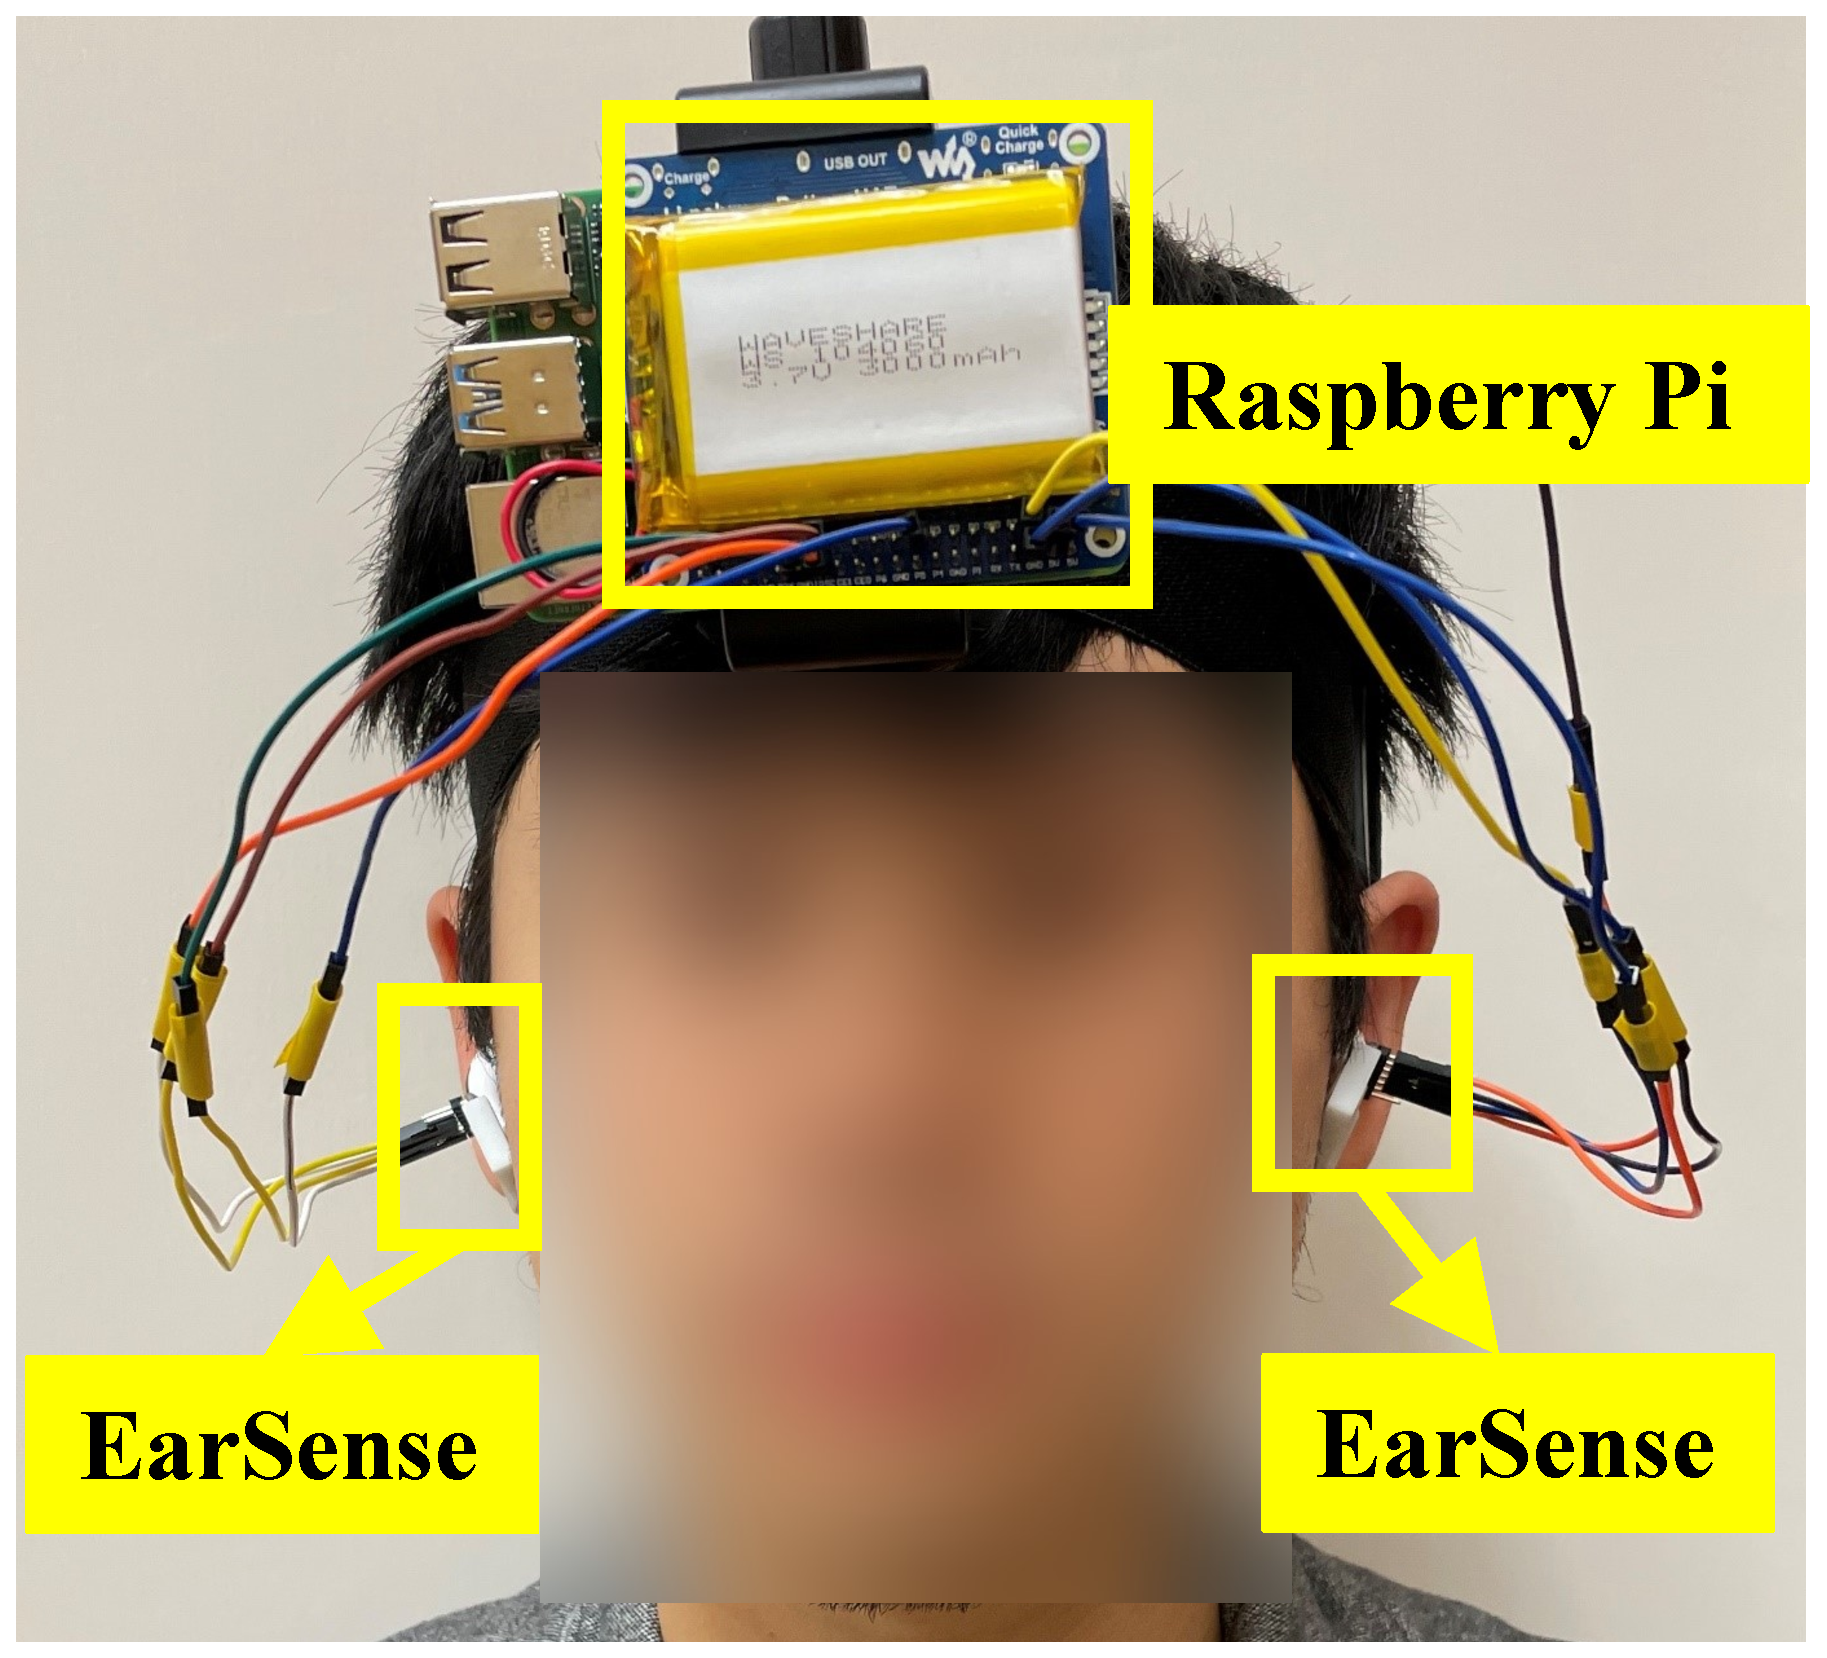
\includegraphics[width=\textwidth]{chapters/vibvoice/figure/people.eps}
    \caption{Test Setup.}
    \label{fig:vibvoice_earsense-people}
  \end{subfigure}
  \caption{\emph{EarSense} is an open-sourced data collector attachable to commercial HMWs for vibration sensing.}
  \label{fig:vibvoice_earsense}
\end{figure}

Fig. \ref{fig:vibvoice_earsense} shows the prototype of \textit{EarSense}  \citep{dataset}, a new open-sourced sensing platform that equips a 3D-printed enclosure with an IMU sensor (i.e., Bosch BMI-160 \citep{Inertial63:online}) inserted. EarSense has a flexible design to make it attachable to any commercial HMW device (e.g., AirPods Pro). EarSense captures the same vibration as the testing HMW and has no direct contact with the user's head (shown in Fig. \ref{fig:vibvoice_earsense-head}).
We connect two EarSenses to a Raspberry Pi (RPi) with a battery for data collection.
Fig. \ref{fig:vibvoice_earsense-people} shows a volunteer wearing the device on the head to avoid excessive vibrations caused by the connecting wires.
A Python script on the RPi to control the EarSense(s) through the I2C protocol and store the data for offline processing. 
We only use the three-axis accelerometer provided by the IMU chip because the gyroscope and magnetometer are less related to the vibration.
The default sample rate of the microphone and the accelerometer are $16\,\text{kHz}$ and $1.6\,\text{kHz}$, respectively. Since commercial earphones like AirPods Pro doesn't support two-channel audio recording, EarSense records audio in a mono channel.
We apply L2-Norm to the spectrograms of three-axis acceleration to extract the vibration intensity and avoid the impact of wearing position and user's motion.

\subsection{Measurements of Bone-Conducted Vibrations}
\label{sec:vibvoice_measurement}
We measure the difference between audio and bone-conducted vibrations with EarSense under various settings, i.e., the noises caused by the competing speaker and user motion. In each experiment, we ask a volunteer to wear Apple AirPods Pro with EarSense attached (shown in Fig. \ref{fig:vibvoice_earsense-people}) in a meeting room with the size of $10~\text{m}^2$. 
\begin{figure}
    \begin{subfigure}{0.46\columnwidth}
        \centering
        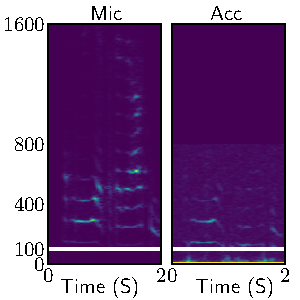
\includegraphics[width=1\textwidth]{chapters/vibvoice/figure/clean.pdf}
        \caption{The user is talking with no noise.}
        \label{fig:vibvoice_nospeaker}
        \end{subfigure}
        \hspace{.5em}
    \begin{subfigure}{0.46\columnwidth}
        \centering
        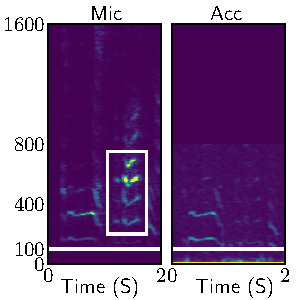
\includegraphics[width=1\textwidth]{chapters/vibvoice/figure/noise.pdf}
        \caption{The user is talking with a competing speaker.}
        \label{fig:vibvoice_speaker}
         \end{subfigure}
    \caption{Impact of the competing speaker.}
    \label{fig:vibvoice_competing-speaker}
\end{figure}

\noindent\textbf{Competing speaker.}
First, we ask the user to sit in the meeting room and speak while a loudspeaker is playing a pre-recording speech one meter from the user as the competing speaker. Note that the competing speaker is one of the most challenging environmental noises for HMWs since its spectrum is similar to the speech's, making it indistinguishable from the noise suppression algorithms. 
We set the volume of the competing speaker to be similar to the user, in which SNR is 3 dB. It is difficult to separate the two sources according to volume since the two speeches are mixed.
Fig. \ref{fig:vibvoice_nospeaker} and Fig. \ref{fig:vibvoice_speaker} show the spectrograms of microphone audio and acceleration when the environment is quiet or contains a competing speaker when the user is talking, respectively.
Note that we only show the spectrogram up to $1.6\,\text{kHz}$ since there is slim energy in the frequency bands higher than $1.6\,\text{kHz}$ of the microphone, and the accelerometer can only sense the signal with a frequency band of $800\,\text{Hz}$.
The spectrograms show that acceleration has lower signal energy than microphone audio since acoustic vibration attenuates during bone conduction, especially for high-frequency vibrations. Compared with the silent environment, the audio spectrogram of microphone audio with a competing speaker shows strong distortions, as highlighted with the white box in Fig. \ref{fig:vibvoice_speaker}. However, the accelerometer spectrograms do not show this phenomenon because the competing speaker cannot produce bone-conducted vibrations.
In summary, the accelerometer receives the user's voice through bone conduction only, excluding environmental sounds over the air, which is ideal for speech enhancement.

\noindent\textbf{User motion.}
We also measure the noises caused by the user's motion. We ask the volunteer to walk while talking. Fig. \ref{fig:vibvoice_walk} shows that walking causes low-frequency noises in the acceleration. The green boxes show the zoom-in result of the signals below $100\,\text{Hz}$. We can observe clear periodic fluctuations in low frequency (i.e., $< 50\,\text{Hz}$), which are caused by the steps of the volunteer.
In summary, the user's motion only affects the acceleration at lower frequencies, which does not affect our speech enhancement.
In addition, we observe slight low-frequency fluctuation in acceleration in Fig. \ref{fig:vibvoice_competing-speaker}, although the volunteer is asked to stand still in this experiment. Since most of the human speech is above $85~\text{Hz}$ \citep{Voicefre75:online}, the removal of audio in low frequency (i.e., the white horizontal lines in Fig. \ref{fig:vibvoice_competing-speaker}) can effectively reduce the interference caused by human motion.

\begin{figure}
\begin{minipage}[t]{0.46\columnwidth}
     \centering
        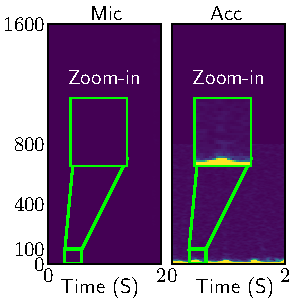
\includegraphics[width=1\textwidth]{chapters/vibvoice/figure/notalk.pdf}
        \caption{Spectrograms of microphone and acceleration when the user is walking.}
        \label{fig:vibvoice_walk}
\end{minipage}
\hfill
   \begin{minipage}[t]{0.48\columnwidth}
     \centering
       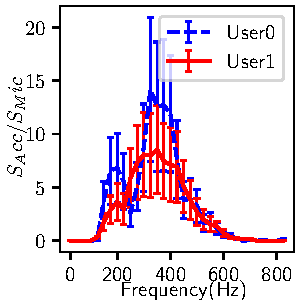
\includegraphics[width=1\textwidth]{chapters/vibvoice/figure/transfer_variance.pdf}
    \caption{Frequency responses of two users' bone-conducted vibrations.}
    %\vspace{-2em}
    \label{fig:vibvoice_bcf}
\end{minipage}
\end{figure}

\noindent\textbf{Frequency Response.}
We further explore the frequency response of bone-conducted vibrations among users. 
Specifically, we measure the frequency response of bone-conducted vibrations as follows: First, we compute the spectrums of audio and vibration data, which is denoted by $S_{Mic}$ and $S_{Acc}$, respectively. Then, we compute the Bone Conduction Function denoted by the frequency response of bone-conducted vibrations by $S_{Acc}/S_{Mic}$ at every frequency band. Fig. \ref{fig:vibvoice_bcf} shows two volunteers' frequency responses, in which the error bars represent the averages and variances.
The acceleration shows higher sensitivity than the microphone within the frequency of $200\text{Hz}\sim500\text{Hz}$, while lower sensitivity at a higher frequency ($>500\text{Hz}$) due to the absorption by the head skull. 
In addition, the frequency response keeps significant similarity among users, indicating the generalization to other users.
Hence, the Bone Conduction Function should consider inter-people diversity and inter-people similarity.

\begin{figure}
\begin{minipage}[t]{0.48\columnwidth}
     \centering
    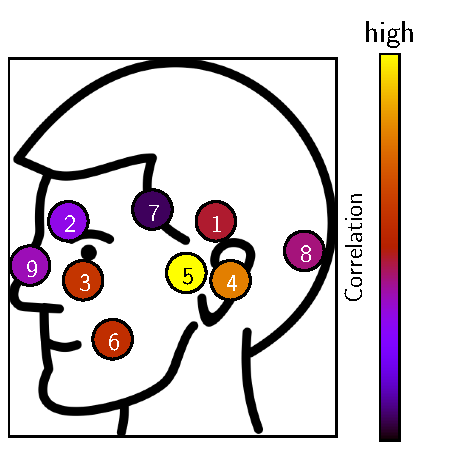
\includegraphics[width=\textwidth]{chapters/vibvoice/figure/correlation.pdf}
    \caption{Intensities of received bone-conducted vibrations on ten locations of the head.}
    \label{fig:vibvoice_head_positison}
\end{minipage}
\hfill
   \begin{minipage}[t]{0.48\columnwidth}
     \centering
    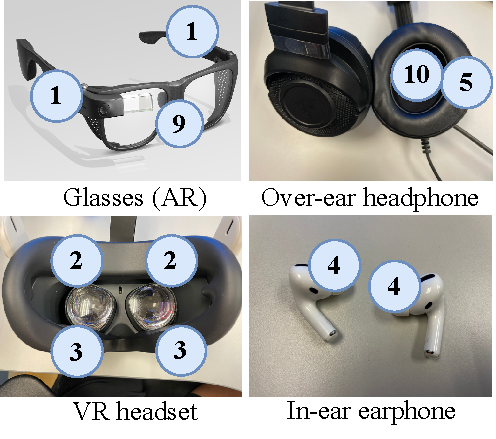
\includegraphics[width=\textwidth]{chapters/vibvoice/figure/devices.pdf}
    \caption{Potential placements on devices.}
    \label{fig:vibvoice_devices}
\end{minipage}
\end{figure}
\noindent\textbf{Locations on the head.}
Bone-conducted vibration exists at various locations on the head. 
As shown in Fig. \ref{fig:vibvoice_head_positison}, we select ten unique locations of interest on the head and measure the intensities of received bone-conducted vibrations. In particular, the nine locations are \#1 \emph{upper ear}, \#2 \emph{eyebrow}, \#3 \emph{cheekbones}, \#4 \emph{ear}, \#5 \emph{temporomandibular joint}, \#6 \emph{cheek}, \#7 \emph{temple}, \#8 \emph{back of the head}, and \#9 \emph{nose}. In addition, we tape EarSense on the interior of the pad of an over-ear headphone, which is denoted as \#10.
Among those positions, some are compatible with commercial HMWs like glasses, headphones, and VR headsets. Fig. \ref{fig:vibvoice_devices} illustrates the corresponding positions on HMWs. The numbers on the HMWs correspond to the locations in Fig. \ref{fig:vibvoice_head_positison}. 
We attach EarSense to the HMWs (when applicable) or on the face for all the following tests. 
We compute Pearson correlation coefficients between the audio and the acceleration on each location and mark the values using a color map in Fig. \ref{fig:vibvoice_head_positison}.
We observe that bone-conducted vibrations exist at most locations of the head. In particular, locations closer to the mouth show higher correlations, indicating a larger possibility of extracting clean speech. 

In summary, our measurements show that bone-conducted vibration has the following characteristics: a) Bone-conducted vibration is robust to environmental voice and only captures the user's speech; b) The user's motion only generates vibrations lower than $85\,\text{Hz}$; c) Bone-conducted vibration has suppressed low and high-frequency audio, which varies across users and within the same user; and d) We can receive audio from multiple locations on the head.



\subsection{Overview of VibVoice}
\label{sec:vibvoice_overview}
\begin{figure*}
  \centering
  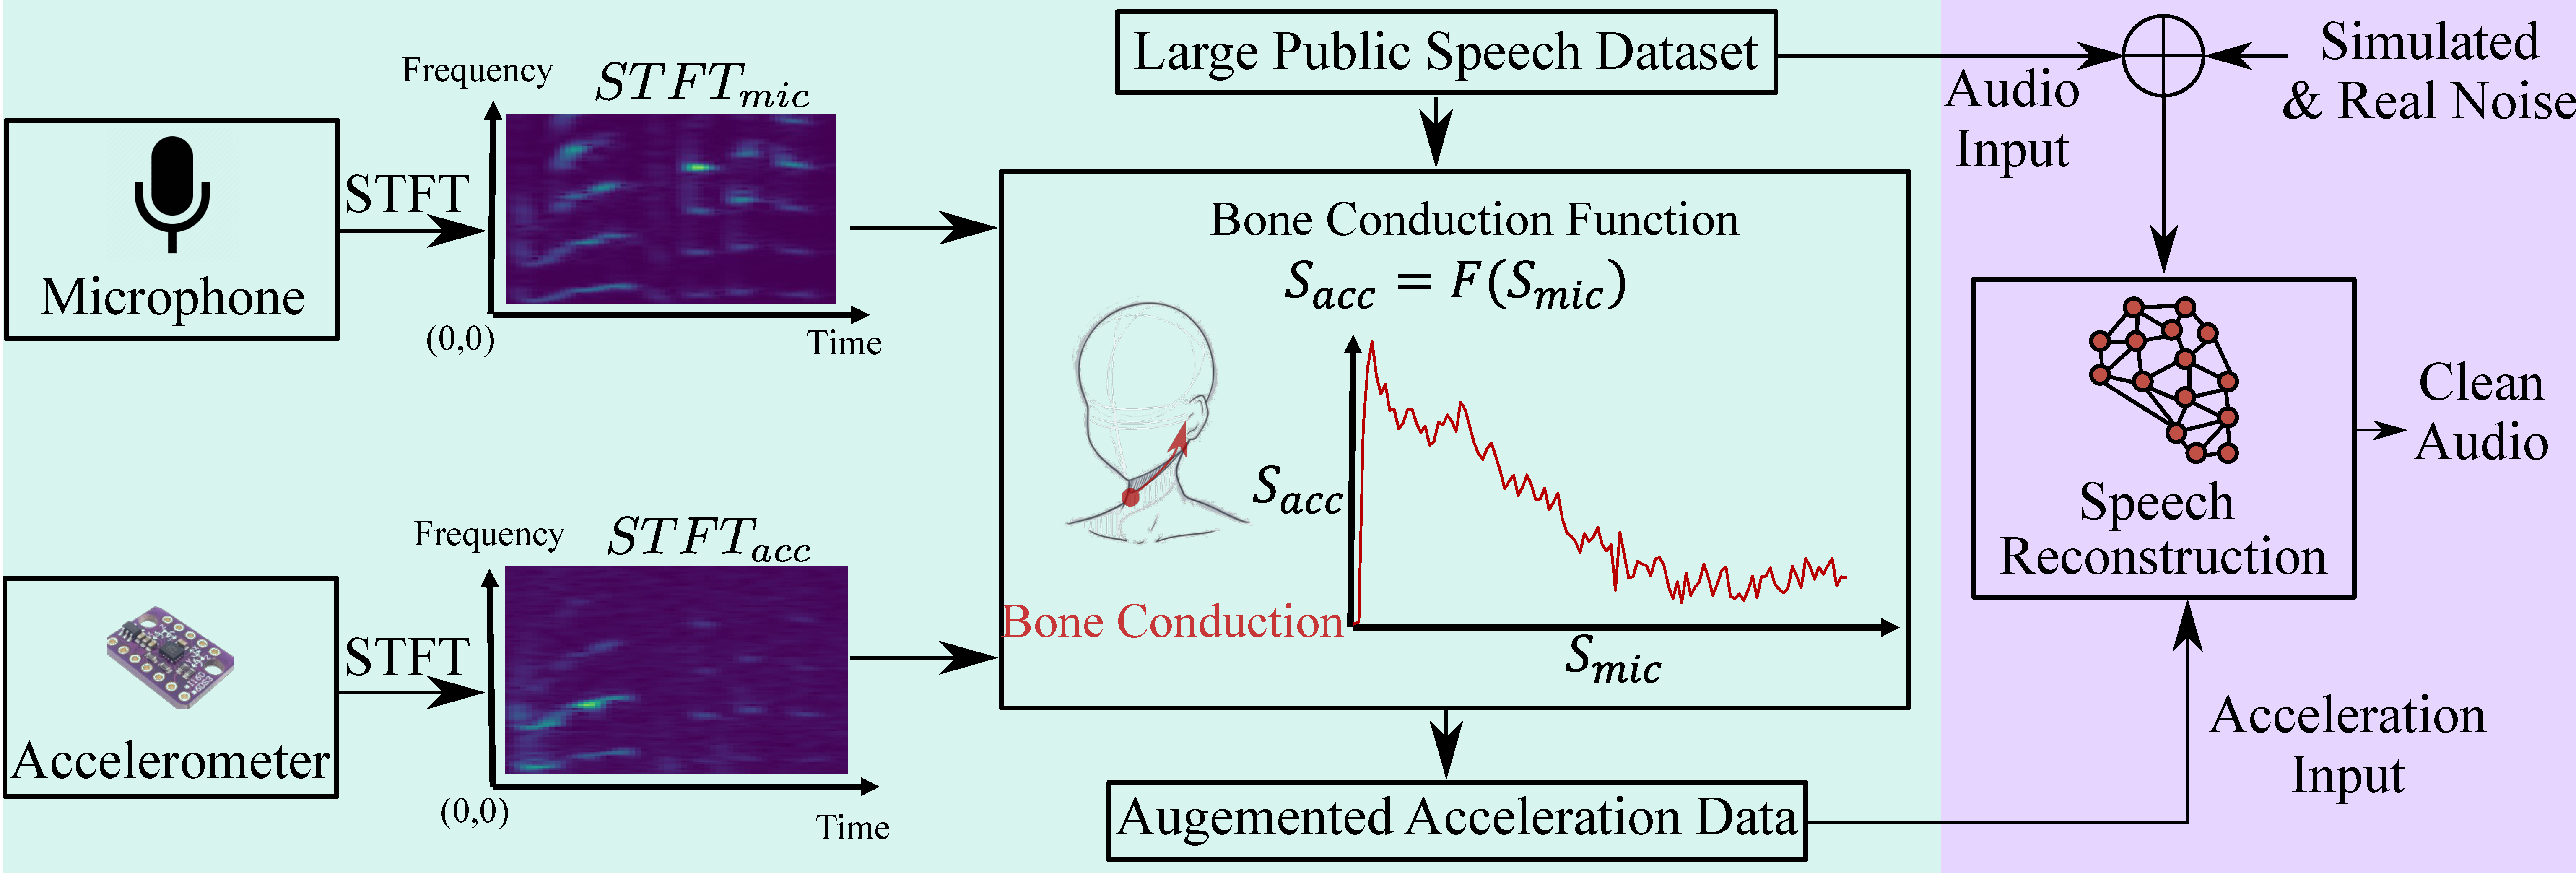
\includegraphics[width=.85\textwidth]{chapters/vibvoice/figure/overview.pdf}
  \caption{The overview of \textit{VibVoice} system. We first augment the acceleration data using a large public speech dataset with estimated Bone Conduction Functions (e.g., the greed box). Then, we train a multi-modal DNN for speech reconstruction (e.g., the purple box).}
  \label{fig:vibvoice_overview}
\end{figure*}
Motivated by our findings in Section. \ref{sec:vibvoice_measurement}, bone-conducted vibration is a promising complementary sensing modality to microphone recording for speech enhancement under environmental noises. 
However, the limited sample rate of HMW's accelerometer and diverse frequency responses of bone-conducted vibration introduce challenges for multi-modal speech enhancement. 
On the other hand, although it is possible to adapt existing audio-only DNN-based speech enhancement models \citep{michelsanti2021overview,sun2021ultrase, zhang2021sensing,liu2021wavoice, ozturk2021radiomic} to take both inputs, there is no large dataset with paired acceleration and audio on HMWs available.

We design \textit{VibVoice}, a speech enhancement system for HMWs that leverages both the microphone recording and the speech information from the bone-conducted vibrations.
Fig. \ref{fig:vibvoice_overview} overviews the design of VibVoice, which contains three components: estimation of Bone Conduction Function, data augmentation, and speech reconstruction network.
% The system overview is shown in Fig. \ref{fig:vibvoice_overview}. 
First, we estimate a set of Bone Conduction Functions using a small paired acceleration-audio dataset collected from volunteers in Section. \ref{sec:vibvoice_function}. 
We note that this estimation does not resort to black-box deep learning approaches, which require a huge amount of training data. Instead, we take advantage of prior knowledge that a frequency response exists between the acceleration and audio spectrograms. 
Then, we augment the acceleration data using the public audio dataset \textit{LibriSpeech} \citep{panayotov2015librispeech} with Bone Conduction Functions in Section. \ref{sec:vibvoice_aug}.
Finally, after generating a large amount of paired acceleration-audio dataset, we train a DNN model which can reconstruct the clean audio from microphone audio and the acceleration data in Section. \ref{sec:vibvoice_network}. 

\subsection{Bone Conduction Function}
\label{sec:vibvoice_bcf}
\subsubsection{Function Formulation}

Measurements in Section. \ref{sec:vibvoice_measurement} show that the acceleration contains acoustic vibrations caused by bone conduction effects. There are two characteristics of acoustic vibrations: a limited sample rate up to $800~\text{Hz}$ and diverse amplitude suppression levels at frequency bands. We model the vibration sensed by the accelerometer as follows: 
\begin{equation}
  s_{acc} = f(s_{mic}) + \epsilon_{acc}=f(s_{speech} + \epsilon_{mic}) + \epsilon_{acc},
  \label{math:transfer_function}
\end{equation}
where $s_{acc}$ and $s_{mic}$ are the raw data captured by the accelerometer and the microphone, respectively; $s_{speech}$ denotes the ground-truth (clean) speech audio; $\epsilon_{acc}$ and $\epsilon_{mic}$ are environmental noises captured by the accelerometer and the microphone, respectively; and $f$ is the Bone Conduction Function.

\subsubsection{Function Estimation}
\label{sec:vibvoice_function}
To estimate the Bone Conduction Function, we recruit volunteers and record a five-minute speech for each person with EarSense and AirPods Pro. The volunteers are asked to read from a daily conversation material \citep{Everyday75:online} in a silent environment. We split paired data into 5-second windows, and each window can contribute one Bone Conduction Function.

First, we compute the spectrograms $STFT_{acc}$ and $STFT_{mic}$ of $s_{acc}$ and $s_{mic}$ for each window using short-time Fourier transform (STFT), respectively.
Then, we apply Otsu's method \citep{otsu1979threshold} to $STFT_{acc}$ and $STFT_{mic}$ for automatic image thresholding, and then discard the bins whose value is lower than a threshold to remove outlier noises.
We note that our thresholding setting can leverage temporal information, which can better diminish the noise than a constant threshold on the frequency or time domains.
Furthermore, we perform the pixel-wise division between $STFT_{acc}$ and $STFT_{mic}$ to obtain a response spectrogram, selecting the lower frequency part of the audio spectrogram to align to the acceleration spectrogram. 
We model the Bone Conduction Function using the Gaussian distribution in the frequency domain since the frequency response (as shown in Fig. \ref{fig:vibvoice_bcf}) has a non-trivial variance due to the complex structure of the head skeleton \citep{chang2016development}. 
In particular, we compute $f=S_{acc}/S_{mic}$ for the corresponding time window in $STFT_{acc}$ and $STFT_{mic}$, respectively. The function $f\sim N(\mu,\sigma^2)$, in which $\mu$ and variance $\sigma$ contribute to the contour and fluctuation of frequency response, respectively.
We measure $\mu$ and $\sigma$ for each time window to construct the parameter pool of Bone Conduction Functions. 

\subsubsection{Data Augmentation with Bone Conduction Functions}
\label{sec:vibvoice_aug}
\begin{figure}
    \centering
    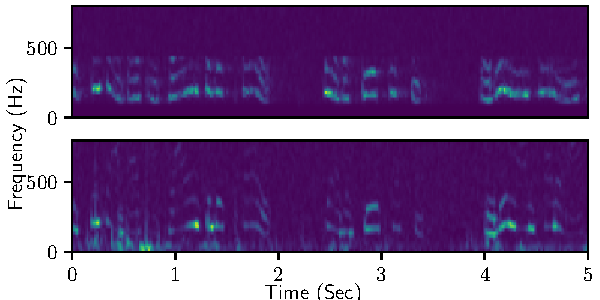
\includegraphics[width=0.35\textwidth]{chapters/vibvoice/figure/synthetic_compare.pdf}
    \caption{Augmented (upper) and real (lower) Acceleration.}
    %\vspace{-1em}
    \label{fig:vibvoice_synthetic_compare}
\end{figure}
We develop a data augmentation approach with Bone Conduction Functions described in Section. \ref{sec:vibvoice_function}.
Note that we cannot apply the inverse Bone Conduction Function to turn the acceleration back to audio due to the significantly limited sample rate of acceleration data. In addition, the frequency band (larger than $500\,\text{Hz}$) has very slim energy, which can cause unreasonable large energy after the inversion.
We utilize these functions to generate acceleration signals using a large-scale audio dataset, i.e., LibriSpeech \citep{panayotov2015librispeech}. 
To be specific, for each audio clip, we first select a Bone Conduction Function (i.e., a list of means and variances over different frequencies) from the pool randomly. 
Then, we restore the frequency response from the Gaussian distribution of given parameters. 
Lastly, we can augment the audio to synthetic acceleration data by directly multiplying the frequency response. 

Fig. \ref{fig:vibvoice_synthetic_compare} shows the spectrograms of augmented acceleration and real acceleration signals, respectively. The augmented spectrogram is close to the real acceleration spectrogram. 
We compute the similarity by calculating the mean of the absolute distance of all pixels in the whole spectrogram and divide it by the largest value of the real acceleration spectrogram. The average error for all volunteers is only 4.5\%, which indicates that our proposed acceleration augmentation is reliable. 

\subsection{Multi-Modal Speech Reconstruction}
\label{sec:vibvoice_network}
Since the sample rate of the microphone is $16\,\text{kHz}$ while the accelerometer is only $1.6\,\text{kHz}$. The reconstruction of high-quality audio from acceleration is an ill-posed task since it requires predicting the lost patterns of the high-frequency band.
Moreover, as we have already generated a large-scale paired acceleration-audio dataset, we can unleash the strong feature extraction capability of DNNs for training. Compared with hand-crafted signal processing approaches, deep learning is robust to diverse inputs. Specifically, we adapt the multi-modal fusion paradigm \citep{sun2021ultrase, zhang2021sensing} and encoder-decoder architecture based on U-net \citep{ronneberger2015u} to build the deep learning model. 
Fig. \ref{fig:vibvoice_CNN} overviews of the DNN design, which is described in detail as follows.


\begin{figure}[tbp]
  \centering
  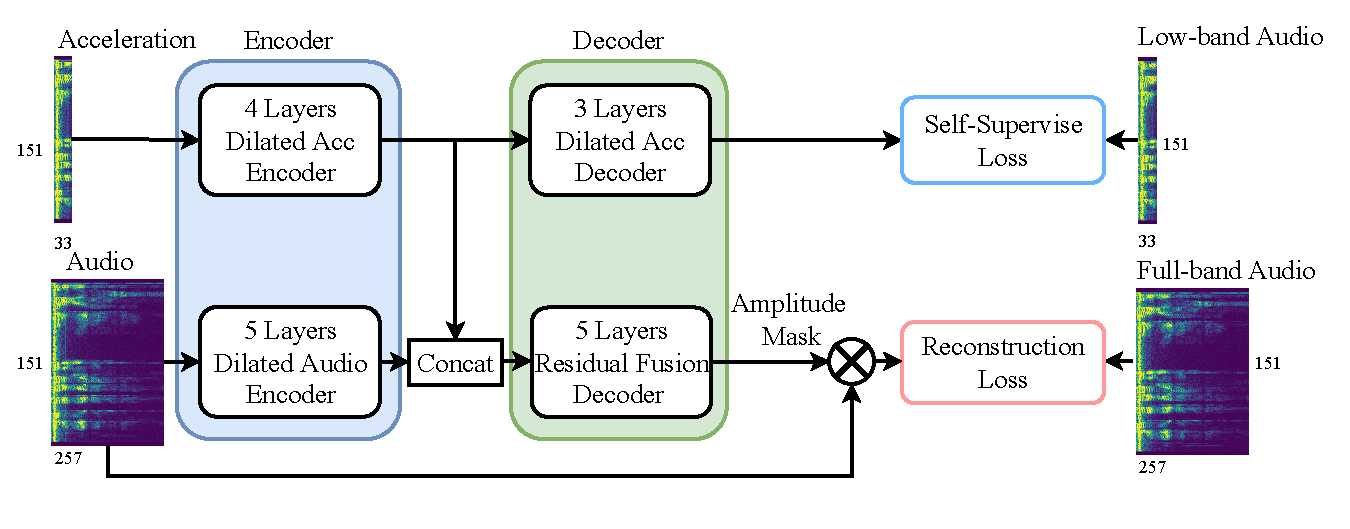
\includegraphics[width=.5\textwidth]{chapters/vibvoice/figure/network.pdf}
  %\vspace{-2em}
  \caption{Overview of our proposed multi-modal network for speech enhancement.}
  \label{fig:vibvoice_CNN}
\end{figure}

\begin{table}[ht!]
\centering
\begin{subtable}[t]{0.5\textwidth}
\centering
\begin{tabular}{lccccccc}\toprule
& \multicolumn{4}{c}{Encoder} & \multicolumn{3}{c}{Decoder}
\\\cmidrule(lr){2-5} \cmidrule(lr){6-8}
Layer & 1 & 2 & 3 & 4 & 1 &2 &3 \\\midrule
Filters &16 &32&64&128 & 64&32 & 16\\ 
Kernel &3 &3&3&3&3&3&3\\ 
Scale &1 &1&0.5&0.5&1&2&2\\
\bottomrule
\end{tabular}
\caption{\label{table1}Acceleration branch.}
\end{subtable}

\begin{subtable}[t]{0.5\textwidth}
\begin{tabular}{lcccccccccc}\toprule
& \multicolumn{5}{c}{Encoder} & \multicolumn{5}{c}{Decoder}
\\\cmidrule(lr){2-6} \cmidrule(lr){7-11}
Layer  & 1 & 2 & 3 & 4 & 5 & 1 &2 &3 &4 & 5  \\\midrule
Filters &16 &32&64&128&256& 128 &64 & 32 & 16 & 1 \\ 
Kernel &3 &5&5&5&5&5& 5 &5 & 5 &3\\ 
Scale &0.5 & 0.5 &0.5 &0.5 & 0.5 & 2 &2 & 2 & 2 & 2\\
\bottomrule
\end{tabular}
\caption{\label{table2}Audio branch.}
\end{subtable}
\caption{{The design of DNN for multi-modal speech reconstruction.}}
\end{table}

\subsubsection{\textbf{Architecture}}
Table \ref{table1} and \ref{table2} show the hyperparameters of our multi-modal neural network of the acceleration and audio branches, respectively. The details are illustrated as follows.

\noindent\textbf{Encoder}.
We use two convolutional networks (CNNs) to encode the high-level features from the two modalities, respectively. Then, we concatenate the features from two encoders along the channel dimension. We stack basic blocks to construct the encoder, where each block consists of a 2D convolutional layer, batch normalization, ReLU activation, and max-pooling. We also design a residual shortcut of the block input before the last deconvolution layer to expedite the training. The filters increase when the layer gets deeper to extract more diverse features. To increase the reception field to capture the harmonic pattern of the whole spectrogram, we use dilated convolution rather than the conventional one.
Since the sample rate of audio data (i.e., $16\,\text{kHz}$) is ten times higher than that of the acceleration data ($1.6\,\text{kHz}$), the size of the audio spectrogram on the frequency axis is also ten times larger. We note that the feature maps from the two modalities should have the same shape at the end of the encoders. Therefore, we discard the parts of the audio spectrogram whose frequency is higher than $6.4\,\text{kHz}$, making the remaining audio frequency band exactly eight times larger than the acceleration data (i.e., $0.8\,\text{kHz}$). In addition, the audio subnet (i.e., encoder) has three more down-sample operations than the acceleration branch to make the output sizes of the two modalities' features consistent. 

\noindent\textbf{Decoder}.
We design two decoders: a fusion decoder and an auxiliary decoder. The decoder has the same design of blocks as the encoder, but the stacked blocks have a decreasing number of filters but increasing sizes of the output tensor. 
The fusion decoder receives both modalities' features via a concatenation and outputs a spectrogram mask. To obtain the constructed clean spectrogram, this mask will be overlaid on the original noisy audio spectrograms by element-wise multiplication. 
The auxiliary decoder only receives the feature of the accelerometer and predicts the low-frequency part of clean audio. The self-supervised loss can prevent the acceleration encoder from being dominated by the audio input, given that the noisy input audio is similar to the clean audio to acceleration by nature (i.e., both are audio).

\subsubsection{\textbf{Waveform reconstruction}}
After obtaining the enhanced spectrogram from the multi-modal decoder, the last step is converting the spectrogram to the waveform using inverse short-time Fourier transform (ISTFT). The DNN of VibVoice only reconstructs the magnitude of the spectrogram. Since the phase of the speech spectrogram is hardly predictable, we use the same phase of the noisy audio signal for the output. Our insight is that although the audio phase can be polluted in a noisy environment, our reconstructed magnitude can attenuate the unwanted time-frequency pixels in spectrograms, which restricts the interference of the noisy phase. Although several works \citep{sun2021ultrase,zhang2021sensing} try to estimate the clean phase by a subnet or a pre-defined algorithm, our tests show that the predicted phase is unstable, and their improvements are marginal and computationally expensive.

\subsubsection{\textbf{Model Training}}
\label{sec:vibvoice_training}
We generate a pool of Bone Conduction Functions by performing cubic interpolation on existing functions from our dataset. We use Gaussian distribution to alleviate our model's overfitting and improve the generalizability among users. In addition, we augment the data with Gaussian distribution based on each frequency band to preserve the low-pass features.
Thus, the limited Bone Conduction Functions can augment a large acceleration-audio dataset from an existing public dataset with diverse features. This dataset can extract the basic features of multiple modalities, but it is not enough for deployment because of the difference between the target user and our pool of Bone Conduction Functions. 
Therefore, we collected another acceleration-audio paired dataset from a different group of volunteers to train the model, which is also used to evaluate VibVoice's performance. 
Note that VibVoice does not require any data from the target user either during the Bond Conduction Function estimation or model training.
All evaluations adopt leave-one-out validation. We pick one user as the testing dataset, while the others are regarded as the training dataset. 

Although the training of VibVoice does not require any data from the target user, one-shot data from the target domain can further improve the overall performance. This data collection can share the recorded data during the setup of HMWs, e.g., the personalized model for calling voice assistants, which incurs no extra overhead to the user. In addition, VibVoice can record data when the user is speaking in a quiet environment. As the data collection doesn't require specific content, our system can unobtrusively record user-specific data during the long-time usage of HMWs and improve the performance of the target user continuously. 

The fusion decoder uses the STFT Loss \citep{defossez2020real}. We use $y$ and $\hat{y}$ to represent the clean and enhanced signals. The STFT loss can be denoted as follows: 
\begin{align} 
\label{math:stft_loss}
\begin{split}
    L_{stft}(y, \hat{y}) &= L_{sc}(y, \hat{y}) + L_{mag}(y, \hat{y}),
    \\
    L_{sc}(y, \hat{y}) &= \frac{||STFT(y)| - |STFT(\hat{y})||_{F}}{||STFT(y)||_{F}},
    \\
    L_{mag}(y, \hat{y}) &= \frac{1}{T}|log|STFT(y)| - log|STFT(\hat{y})||_{1},
\end{split}
\end{align} 
where $L_{sc}$ refers to convergence
(sc) loss and $L_{mag}$ refers to the magnitude (mag) loss.
We use Mean Square Error (MSE) as the training loss for the auxiliary decoder. The fusion decoder and auxiliary decoder targets are full-band clean spectrogram and lower-band clean spectrogram, respectively. The final loss is formulated as follows: 
\begin{align} 
\label{math:overall_loss}
\begin{split}
    L(y, \hat{y}) &= L_{stft}(y, \hat{y}) + |y_{lowband} - \hat{y}_{lowband}|_{2} \times \lambda,
\end{split}
\end{align}
which is the joint loss function that covers both fusion and auxiliary decoder. We set $\lambda$ to 0.05 to balance the scales of two losses.

